\chapter{Einleitung} \label{chap:intro}

Im Zentrum des ersten Kapitels steht der Einsatz von \emph{Deep Learning} im Bereich der Umweltbeobachtung. Es werden auch Fragestellungen aufgeführt, die einen Überblick über den Aufbau der Arbeit geben.

\section{Deep Learning in der Umweltbeobachtung}

Der \emph{LOEWE-Schwerpunkt Natur 4.0 Sensing Biodiversity} (abgekürzt: Natur 4.0) ist ein Gemeinschaftsprojekt der federführenden Philipps-Universität Marburg, der Justus-Liebig-Universität Gießen, der Technische Universität Darmstadt und der Senckenberg Gesellschaft für Naturforschung in Frankfurt. Ziel des Projekts ist die Entwicklung eines Umweltmonitoringsystems zur hoch aufgelösten Beobachtung von naturschutzrelevanten Arten, Lebensräumen und Prozessen durch vernetzte Sensorik und integrative Datenanalyse\footfullcite{LOEWE-Natur4.0}. Das Testgebiet für die Prototypentwicklung von Natur 4.0 ist der Marburger Universitätswald in Caldern. 

Einer der Schwerpunkte des Projekts liegt auf \textbf{der visuellen Erkennung von Tierarten}. Die Ergebnisse dieser Aufgabe ermöglichen zusammen mit weiteren zeitlichen und räumlichen Sensordaten die Beantwortung folgender Fragen: Welche Tierarten sind im Testgebiet vorhanden? Wann, wie häufig, wo genau und unter welchen Bedingungen kommen sie vor? Antworten auf diese Fragestellungen erweisen sich als wertvoll: Sie geben nicht nur Auskunft über die biologische Vielfalt und Eigenschaften von Ökosystemen im Testgebiet, sondern auch über die Wechselwirkungen zwischen Tieren, Pflanzen und klimatischen Bedingungen darin. Aus solchen Informationen lassen sich verschiedene Naturschutzstrategien ableiten.

Bei einem gegebenen Bild gilt die visuelle Erkennung von Tierarten als erfolgreich, wenn alle Tiere in diesem Bild gefunden und richtig kategorisiert werden. Die Aufgabe ist in der Tat ein typisches Beispiel für \emph{das Objekterkennungsproblem}.

\subsection{Objekterkennung}

Die Objekterkennung im Forschungsfeld \emph{Computer-Vision} erfolgt in zwei Schritten:

\begin{enumerate}
	\item \emph{Objektlokalisierung}: Der erste Schritt bezieht sich auf das Identifizieren der Position eines oder mehrerer Objekte in einem Bild und das Zeichnen eines Begrenzungsrahmens um ihre Ausdehnung.
	
	\item \emph{Bildklassifizierung}: Bei dem zweiten Schritt handelt es sich um die Aufgabe, einem Bildobjekt ein Label aus einem festen Satz von Kategorien zuzuweisen.
\end{enumerate}

Auf die gleiche Weise lässt sich die visuelle Erkennung von Tierarten erledigen. Die Tiere im Eingabebild müssen zunächst lokalisiert und anschließend klassifiziert werden, um als richtig erkannt zu gelten.

Man verwendet \emph{den datengetriebenen Ansatz}, um das Objekterkennungsproblem zu lösen. Die Idee dabei ist, dem Computer viele Bilder jeder einzelnen Objektklasse bereitzustellen und dann mit dem Computer Lernalgorithmen zu entwickeln (\emph{trainieren}), die sich diese Bilder ansehen und visuelle Merkmale lernen, die Objekte von ihrer Umgebung und jede Klasse voneinander trennen. Ergebnis der Lernphase ist ein \emph{trainiertes Modell}, das aus Bilddaten im Rahmen des Projekts Natur 4.0 bestimmte Tierarten erkennen können soll.

Die zu entwickelnden Algorithmen im datengetriebenen Ansatz fallen unter die Kategorie \emph{Deep-Learning-Algorithmen}, die die Lernfähigkeit von Computern ermöglichen.

\subsection{Deep Neural Network}

In der Regel besteht ein Deep-Learning-Algorithmus (im Weiteren als \emph{Deep Neural Network} (DNN) bezeichnet) aus einer \emph{Eingabeschicht}, einer \emph{Ausgabeschicht} und mindestens zwei \emph{verborgenen Schichten}. Jede Schicht setzt sich aus \emph{Neuronen} zusammen, die Informationen von anderen Neuronen oder von außen aufnehmen, modifizieren und als Ergebnis ausgeben. Jedes Neuron ist mit allen anderen Neuronen in der vorherigen sowie nächsten Schicht verbunden (siehe \autoref{fig:DNN}). Jeder Verbindung wird ein Gewicht zugewiesen.

\begin{figure}[!hb]
	\centering
	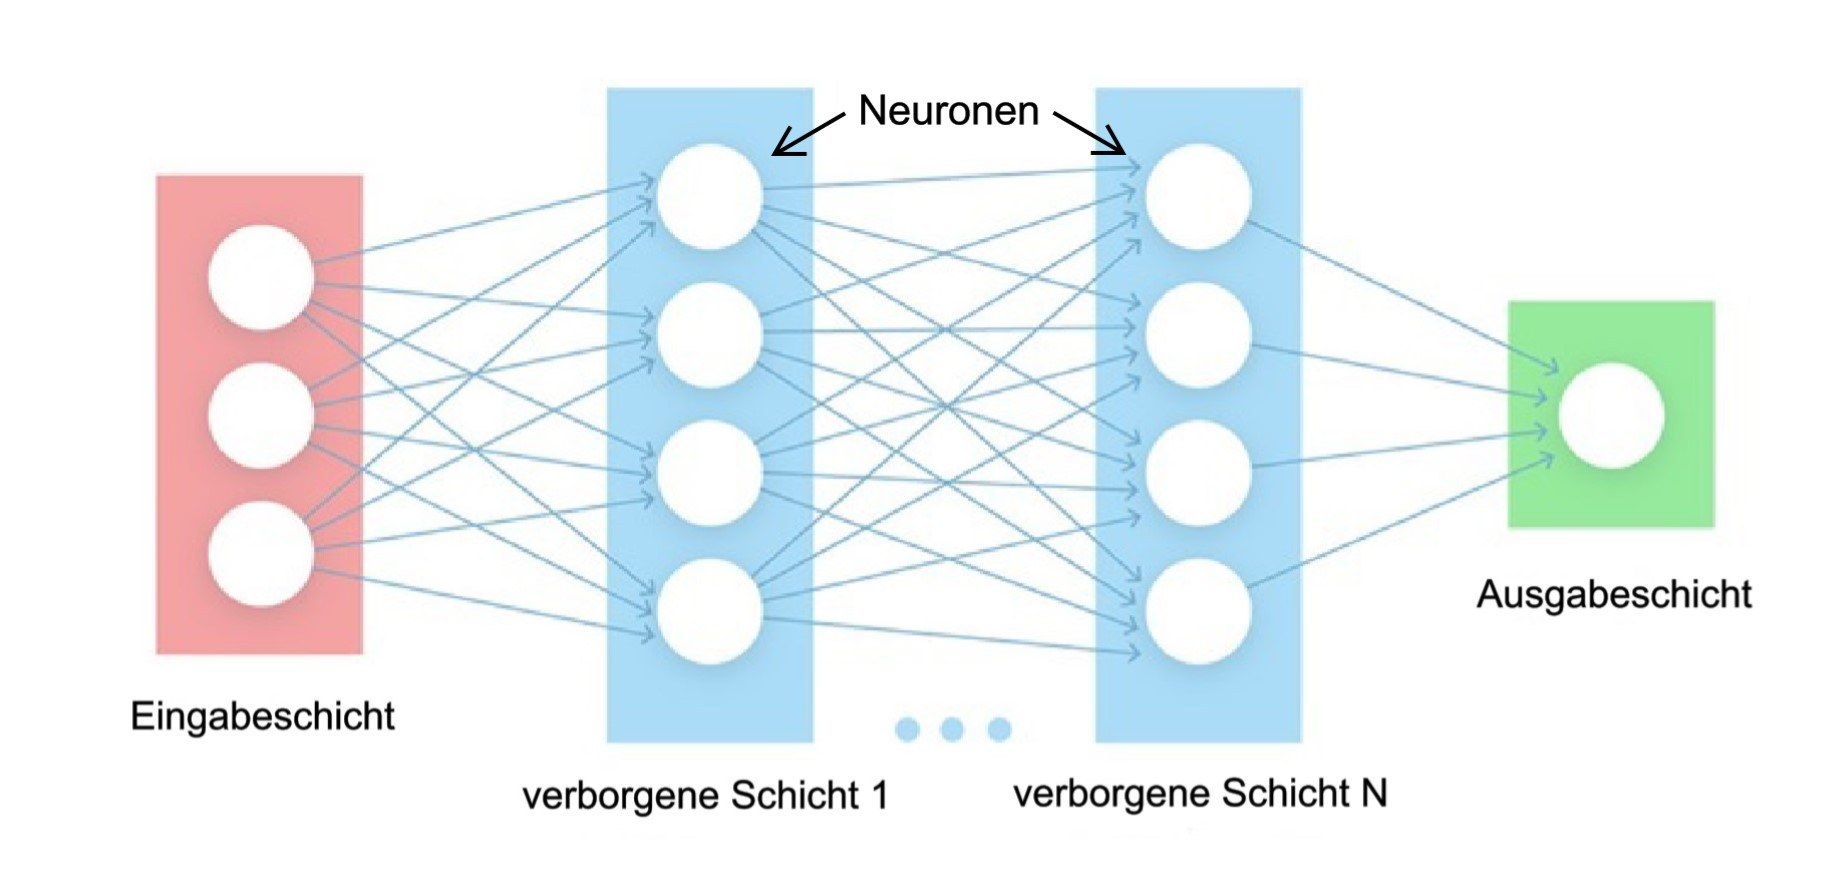
\includegraphics[width=\linewidth]{images/DNN}
	\caption{Aufbau eines Deep Neural Network \protect\cite{AufbauDNN}}
	\label{fig:DNN}
\end{figure}

DNNs lassen sich mittels des \emph{Backpropagation-Algorithmus} \cite{backpropapaper,Goodfellow-et-al-2016} trainieren. Der Algorithmus speist zunächst jede Trainingsinstanz in das zu trainierende DNN ein und berechnet die Ausgabe jedes Neurons in jeder konsekutiven Schicht (\emph{Vorwärtsdurchlauf}). Danach ermittelt er den Ausgabefehler des DNN (i.~e., die Differenz zwischen der gewünschten und der tatsächlichen Ausgabe), durchläuft jede Schicht in umgekehrter Richtung, um den Fehlerbeitrag jeder Neuronenverbindung auszurechnen (\emph{Rückwärtsdurchlauf}), und schließlich optimiert die entsprechenden Verbindungsgewichte, um den Ausgabefehler des DNN zu minimieren, was das Ziel des gesamten Trainingsprozesses ist.

Für die Objekterkennung verwendet man einen bestimmten Typ von DNN namens \emph{Convolutional Neural Network} (CNN) (mehr dazu im \autoref{chap:cnn}). Unterschiedliche CNNs haben unterschiedliche Anordnungen von Schichten unterschiedlicher Typen (Architekturen), jedoch die gleiche Funktionsweise: CNNs konzentrieren sich auf \emph{Low-Level-Merkmale} in den ersten Schichten und setzen diese anschließend in den nächsten zu \emph{Higher-Level-Merkmale} zusammen. Beispielweise kann der Computer in niedrigeren Schichten lernen, Kanten oder Linien oder auch Kurven aus Pixel der Eingabebilder zu identifizieren, während er in höheren Schichten komplexere Formen sowie visuelle Merkmale lernt, die für die Objekterkennung ausschlaggebend sind.

Als Indikator für den Fortschritt in der Entwicklung von CNNs im Bereich Computer-Vision können die Metriken Top-1- bzw. Top-5-Genauigkeit vom Wettbewerb \emph{ImageNet Large Scale Visual Recognition Challenge} (ILSVRC) \cite{russakovsky2015imagenet} herangezogen werden. In ILSVRC werden Modelle (Implementierungen theoretischer Architekturen) mit der Bildklassifizierung des \emph{ImageNet-Datensatzes} beauftragt, der tausend nicht überlappende Klassen und insgesamt ca. 1,35 Millionen Bilder umfasst\footnote{Tatsächlich ist der zu klassifizierende Datensatz nur eine Teilmenge vom realen ImageNet-Datensatz, der gemäß \cite{ridnik2021imagenet21k} 21\,841 überlappende Klassen umfasst. Zum Unterscheiden wird im Weiteren die Teilmenge als ImageNet(-1K), der reale Datensatz als ImageNet-21K bezeichnet.}. Die Top-K-Genauigkeit stellt den Anteil der Testbilder dar, für die die Top-K-Prognosen des zu testenden Modells die richtige Antwort enthalten. Nach \emph{Papers with Code} \cite{PapersWithCode-ImageNet} sind die folgenden Architekturen zum Zeitpunkt dieser Arbeit Stand der Technik im Bereich der Bildklassifizierung:

\begin{enumerate}
	\item \emph{Vision-Transformer} \cite{dosovitskiy2021image} - Beste ImageNet Top-1-Genauigkeit: 90,45\%  \cite{zhai2021scaling}
	\item \emph{EfficientNet} \cite{tan2020efficientnet} - Beste ImageNet Top-1-Genauigkeit: 90,20\%  \cite{pham2021meta}
	\item \emph{ResNet} \cite{he2015deep} - Beste ImageNet Top-1-Genauigkeit: 87,54\% \cite{kolesnikov2020big}
\end{enumerate}

Zur visuellen Erkennung von Tierarten im Projekt Natur 4.0 kann eines der Modelle der aufgeführten Architekturen eingesetzt werden. Der Grund dafür basiert auf dem Konzept von \emph{Transfer Learning}, das im Grunde eine Methode ist, die ein für eine Aufgabe A entwickeltes Modell als Ausgangspunkt für eine andere ähnliche B wiederverwendet. Ein solches Modell könnte bereits Merkmale gelernt haben, die für Aufgabe B relevant oder nützlich sind. Da die aufgeführten Architekturen über Modelle verfügen, die zuvor auf dem ImageNet-Datensatz trainiert wurden, der zahlreiche Tierarten unter seinen tausend Klassen enthält\footfullcite{ImageNet1000Classes}, ist es durchaus möglich, dass diesen Modellen Grundunterschiede zwischen Tierarten schon bekannt sind, d.~h. die Modelle haben mit hoher Wahrscheinlichkeit ihre Gewichte zum Trennen von Tierarten optimiert. Die Verwendung dieser Gewichte anstatt zufällig initialisierter Gewichte kann zur besseren Vorinitialisierung der Modelle dienen, die zur visuellen Erkennung von Tierarten eingesetzt werden. Man kann somit Teile des aufwendigen Trainings überspringen und infolgedessen Zeit sowie Speicher- und Rechenressourcen sparen, denn komplexe CNNs können in der Praxis tage- oder wochenlang von Grund auf trainiert werden \cite[4]{Schroff_2015}\cite[1]{codreanu2017scale}\cite{BBVADeepLearning,StanfordDAWNBench}. 

\section{Die zentralen Fragestellungen}

Die visuelle Erkennung von Tierarten im Projekt Natur 4.0 ist ein Objekterkennungsproblem, das sich mit dem datengetriebenen Ansatz lösen lässt. Damit dieser Lösungsansatz nach dem Transfer-Learning-Konzept umgesetzt werden kann, sind folgende Fragestellungen zu beantworten:

\begin{enumerate}
	\item \textbf{Welche vortrainierte Modelle werden zur visuellen Erkennung von Tierarten im Projekt Natur 4.0 eingesetzt?}
	
	\item \textbf{Wie werden die ausgewählten Modelle implementiert?}
	
	\item \textbf{Welche Leistung können die implementierten Modelle erzielen?}
\end{enumerate}

Antworten auf die aufgeführten Fragestellungen lassen sich der Reihe nach in den \autoref{chap:relatedwork}, \autoref{chap:training} sowie \autoref{chap:experimentresult} finden. Um jedoch die Argumentationen nachzuvollziehen, die zu diesen Antworten geführt haben, wird empfohlen, zunächst die grundlegenden Konzepte von CNN zu verstehen, die im \autoref{chap:cnn} ausführlicher beschrieben sind.